\documentclass[11pt,a4paper]{article}

\usepackage[margin=1in, paperwidth=8.3in, paperheight=11.7in]{geometry}
\usepackage{amsfonts}
\usepackage{amsmath}
\usepackage{amssymb}
\usepackage{dsfont}
\usepackage{enumerate}
\usepackage{enumitem}
\usepackage{fancyhdr}
\usepackage{graphicx}
\usepackage{tikz}
\usepackage{changepage} 

\begin{document}

\pagestyle{fancy}
\setlength\parindent{0pt}
\allowdisplaybreaks

\renewcommand{\headrulewidth}{0pt}

% Cover page title
\title{Machine Learning - Supplement 1}
\author{Dom Hutchinson}
\date{\today}
\maketitle

% Header
\fancyhead[L]{Dom Hutchinson}
\fancyhead[C]{Machine Learning - Supplement 1}
\fancyhead[R]{\today}

% Default enumerate labeling
\setlist[enumerate,1]{label={\roman*)}}

% Counters
\newcounter{definition}[section]
\newcounter{example}[section]
\newcounter{notation}[section]
\newcounter{proposition}[section]
\newcounter{proof}[section]
\newcounter{remark}[section]
\newcounter{theorem}[section]

% commands
\newcommand{\dotprod}[0]{\boldsymbol{\cdot}}
\newcommand{\cosech}[0]{\mathrm{cosech}\ }
\newcommand{\cosec}[0]{\mathrm{cosec}\ }
\newcommand{\sech}[0]{\mathrm{sech}\ }
\newcommand{\prob}[0]{\mathbb{P}}
\newcommand{\nats}[0]{\mathbb{N}}
\newcommand{\cov}[0]{\mathrm{Cov}}
\newcommand{\var}[0]{\mathrm{Var}}
\newcommand{\expect}[0]{\mathbb{E}}
\newcommand{\reals}[0]{\mathbb{R}}
\newcommand{\integers}[0]{\mathbb{Z}}
\newcommand{\indicator}[0]{\mathds{1}}
\newcommand{\nb}[0]{\textit{N.B.} }
\newcommand{\ie}[0]{\textit{i.e.} }
\newcommand{\eg}[0]{\textit{e.g.} }
\newcommand{\X}[0]{\textbf{X}}
\newcommand{\x}[0]{\textbf{x}}
\newcommand{\iid}[0]{\overset{\text{iid}}{\sim}}
\newcommand{\proved}[0]{$\hfill\square$\\}

\newcommand{\definition}[1]{\stepcounter{definition} \textbf{Definition \arabic{section}.\arabic{definition}\ - }\textit{#1}\\}
\newcommand{\definitionn}[1]{\stepcounter{definition} \textbf{Definition \arabic{section}.\arabic{definition}\ - }\textit{#1}}
\newcommand{\proof}[1]{\stepcounter{proof} \textbf{Proof \arabic{section}.\arabic{proof}\ - }\textit{#1}\\}
\newcommand{\prooff}[1]{\stepcounter{proof} \textbf{Proof \arabic{section}.\arabic{proof}\ - }\textit{#1}}
\newcommand{\example}[1]{\stepcounter{example} \textbf{Example \arabic{section}.\arabic{example}\ - }\textit{#1}\\}
\newcommand{\examplee}[1]{\stepcounter{example} \textbf{Example \arabic{section}.\arabic{example}\ - }\textit{#1}}
\newcommand{\notation}[1]{\stepcounter{notation} \textbf{Notation \arabic{section}.\arabic{notation}\ - }\textit{#1}\\}
\newcommand{\notationn}[1]{\stepcounter{notation} \textbf{Notation \arabic{section}.\arabic{notation}\ - }\textit{#1}}
\newcommand{\proposition}[1]{\stepcounter{proposition} \textbf{Proposition \arabic{section}.\arabic{proposition}\ - }\textit{#1}\\}
\newcommand{\propositionn}[1]{\stepcounter{proposition} \textbf{Proposition \arabic{section}.\arabic{proposition}\ - }\textit{#1}}
\newcommand{\remark}[1]{\stepcounter{remark} \textbf{Remark \arabic{section}.\arabic{remark}\ - }\textit{#1}\\}
\newcommand{\remarkk}[1]{\stepcounter{remark} \textbf{Remark \arabic{section}.\arabic{remark}\ - }\textit{#1}}
\newcommand{\theorem}[1]{\stepcounter{theorem} \textbf{Theorem \arabic{section}.\arabic{theorem}\ - }\textit{#1}\\}
\newcommand{\theoremm}[1]{\stepcounter{theorem} \textbf{Theorem \arabic{section}.\arabic{theorem}\ - }\textit{#1}}

\section{Variational Bayes}
\textit{Variational Bayes} is a method for approximating an intractable integral, $P$, with a tractable one, $Q$. This is useful as \textit{Posterior}s are integrals and generally intractable.
$$P(X|Y)\approx Q(X)$$
From the derivation below we get that
$$\ln P(Y)=KL(Q\|P)-\expect_X[\ln Q(X)-\ln P(X,Y)$$
since $\ln P(Y)$ is fixed wrt $Q$ we can derive a likelihood function
$$\mathcal{L}(Q)=-\expect_X[\ln Q(X)-\ln P(X,Y)]$$
If we maximise this likelihood function, $\mathcal{L}$, then we are minimising $KL(Q||P)$ which means $Q$ \& $P$ are becoming similar.\\
We have reduced the problem of approximation to just optimising $\mathcal{L}(Q)$.\\
By choosein g a good form for $Q$ $\mathcal{L}(Q)$ becomes tractable.

\subsection{Kullback-Leibler Divergence}
\textit{Kullback-Leibler Divergence} is a similarity measure for two distributions, $Q\ \&\ P$.
$$KL(Q||P):=\int Q(X)\ln\left(\frac{Q(X)}{P(X|Y)}\right)dX$$
The lower the value of $KL(Q||P)$ the similar $Q$ \& $P$ are.\\
\nb $KL(\cdot||\cdot)\geq 0$ and $KL(Q||Q)=1$.

\subsection{Intractibiltiy}
Here I show why the \textit{Posterior} is intractrable
$$\underbrace{P(X|Y)}_\text{Intractable}=\frac{\overbrace{P(Y|X)P(X)}^\text{Tractable}}{\underbrace{P(Y)}_\text{Intractable}}=\frac{P(Y|X)P(X)}{\underbrace{\int P(X,Y)dX}_\text{Intractable}}$$
$\int P(X,Y)dX$ is intractable since the space $X$ is intractablly large.\\
This makes the evidence, and thus posterior, intractable.

\subsection{Derivation}
\[\begin{array}{rcl}
KL(Q||P)&=&\displaystyle\sum_X Q(X)\ln\left[\dfrac{Q(X)}{P(X|Y)}\right]\\
&=&\displaystyle\sum_X Q(X)\ln\left[\dfrac{Q(X)P(X)}{P(X,Y)}\right]\text{ by product rule}\\
&=&\displaystyle\sum_XQ(X)[\ln Q(X)+\ln P(Y)-\ln P(X,Y)]\text{ by log rules}\\
&=&\expect_X[\ln Q(X)-\ln P(X,Y)]+\ln P(Y)\text{ since }P(Y)\text{ is independent of X}\\
\implies\ln P(Y)&=&KL(Q||P)-\underbrace{\expect_X[\ln Q(X)-\ln P(X,Y)]}_{\mathcal{L}(Q)}
\end{array}\]

\section{Predicitive Gaussian Processes}
\textit{Gaussian Processes} are the class of \textit{Stochastic Processes} st every finite linear combination of random variables is normally distributed.\\
Here I describe the process of make predictions for the value at a set of points, given training data $(X,y)$.
\begin{enumerate}
	\item Observed data points, $(X,y)$.
	\item Define the set of points we wish to predict values at, $(X^*)$.
	\item Define a kernel function to use as the covaraince funtion, $k(\cdot,\cdot)$.
	\item Calculate $\pmb\mu^*,\Sigma^*$ for the points $X^*$, using the equations below.
	\item Draw samples from $\text{Normal}(\pmb\mu^*,\Sigma^*)$. Each sample can be used to infer a function.
\end{enumerate}

\subsection{Equations}
\textbf{Without Noise}
\[\begin{array}{rcl}
\pmb\mu^*&=&k(X^*,X^*)k(X,X)^{-1}y\\
\Sigma^*&=&k(X^*,X^*)-k*X^*,X)k(X,X)^{-1}k(X^*,X)^T
\end{array}\]
\textbf{With Noise}
\[\begin{array}{rcl}
\pmb\mu^*&=&k(X^*,X^*)k(X,X\pmb{+c})^{-1}y\\
\Sigma^*&=&k(X^*,X^*)-k*X^*,X)k(X,X\pmb{+c})^{-1}k(X^*,X)^T
\end{array}\]
The only difference is the $+c$ in the $K(X,X)$ terms.\\
\nb $\pmb\mu^*\in\reals^N\ \&\ \Sigma^*\in\reals^{N\times N}$ where $N:=|X^*|$.

\subsection{Kernels}
\begin{center}
\begin{tabular}{l|l}
Linear&$k(\x,\textbf{y})=\sigma^2\times \textbf{x}^T\textbf{y}$\\
White&$k(\x,\textbf{y})=\sigma^2I$\\
Periodic&$k(\x,\textbf{y})=\sigma^2\text{exp}\left\{-\frac2{\ell^2}\sin^2\left(\frac{\pi}{p}\|\x-\textbf{y}\|\right)\right\}$\\
&\quad where\\
&\quad\quad $\ell=$length scale\\
&\quad\quad $p=$period\\
Radial Basis Function&$k(\x,\textbf{y})=\text{exp}\left\{-\frac{1}{\ell^2}\|\x-\textbf{y}\|^2\right\}$\\
&\quad where\\
&\quad\quad $\ell=$length scale\\
\end{tabular}
\end{center}
Vary $\sigma^2$ depending on noise in readings.\\
\nb $\|\x\|:=\sqrt{\sum x_i^2}\implies\ \|\x-\textbf{y}\|=\sqrt{\sum(x_i-y_i)^2}$. This is the \textit{Euclidean Distance}.

\section{Dirichlet Processes}
\textit{Dirichlet Processes} are the class of \textit{Stochastic Processes} whose realisations are probability distributions.\\
\textit{Dirichlet Processes} take a base distribution, $f(\cdot)$, and a concentration parameter, $\alpha\in\reals$. Realisations become more continuous the greater the value $\lim\alpha$ tends to.\\
\\
The following algorithm is used to construct a realisation
\begin{enumerate}
	\item With probability $\dfrac\alpha{\alpha+n-1}$ draw $X_n$ from $f(\cdot)$.
	\item With probability $\dfrac{n_x}{\alpha+n-1}$ set $X_n=x$\\
	 where $n_x:=|\{j<n:X_j=x\}|$ (\ie the number of previous observations of $x$).
\end{enumerate}
These $X_1,X_2,\dots$ represent the relative frequcies with which each value should occur in the distribution. In practice we cannot produce full distributions as that would require infinite iterations of the algorithm, instead we are just approximating it.\\
\nb $X_1,X_2,\dots$ are not independent since they depend on the previously generated results.\\
\nb The base distribution, $f(\cdot)$, is the expected result.

\section{Ising Model}
An \textit{Ising Model} is one where each latent variable takes one of two states and only has dependency on neighbours in such a way that a grid is formed. Thus dependencies are undirected, forming a \textit{Markov Random Field}.
\begin{center}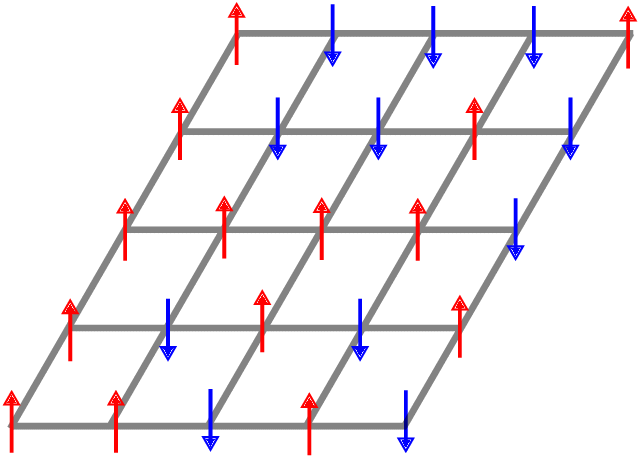
\includegraphics[scale=.2]{img/ising.png}\end{center}

\subsection{Ising Prior}
$$p(\x)=\frac{1}{Z_0}e^{{\displaystyle\sum_{i\in\x}\sum_{j\in N_i}w_{ij}x_ix_j}}$$
where $Z_0$ is a normalising term, $N_i$ is the neighbourhood of $x_i$ \& $w_{ij}$ is the weighting of the relationship between variables $x_i$ \& $x_j$.\\
\nb $x_ix_j=1$ iff $x_i=x_j$, otherwise $x_i,x_j=-1$. Thus this term only increases when $x_i$ has the same value as many of its neighbours.

\subsection{Iterative Conditional Modes}
\textit{Iterative Conditional Modes} is a tecnique for inferring latent variable values in an \textit{Ising Model}.
\begin{enumerate}
	\item Randomly initalise $\x$.
	\item For each $x_i\in\x$.
	\begin{enumerate}
		\item Assume all latent values are fixed except for $x_i$.
		\item Assign $x_i$ to the most likely value given the other values.
	\end{enumerate}
	\item Repeat ii) until time is up
\end{enumerate}

\subsection{Gibbs Sampling}
\textit{Gibbs Sampling} is an implementation of \textit{Markov Chain Monte Carlo}.\\
\\
The general idea is that given a distribution $p(\x)$ which we wish to sample from we shall draw samples from one dimension at a time, using the other dimensions as conditions, $p(x_i|\x_{\neg i})$.\\
\\
If we now just consider the \textit{Ising Model} we can perform some derivations
\[\begin{array}{rcl}
p(x_i|\x_{\neg i},\textbf{y})&=&\dfrac{p(\x,\textbf{y})}{p(\x_{\neg i},\textbf{y})}\\
&=&\dfrac{p(\x,\textbf{y})}{\displaystyle\int p(\x,\textbf{y})dx_i}\\
&=&\dfrac{p(\x,\textbf{y})}{\displaystyle\sum_{x_i\in\{1,-1\}} p(\x,\textbf{y})}\\
&=&\dfrac{p(\x,\textbf{y})}{p(x_i=1,\x_{\neg i},\textbf{y})+p(x_i=-1,\x_{\neg i},\textbf{y})}\\
\implies p(x_i=1|\x_{\neg i},\textbf{y})&=&\dfrac{p(x_i=1\x_{\neg i},\textbf{y})}{p(x_i=1,\x_{\neg i},\textbf{y})+p(x_i=-1,\x_{\neg i},\textbf{y})}\\
\end{array}\]
This is a tractable expression.\\
\\
Here is an algorithm for \textit{Gibbs Sampling}
\begin{enumerate}
	\item Randomly initalise $\x$.
	\item For each $x_i\in\x$.
	\begin{enumerate}
		\item Calculate $p(x_i=1|\x_{\neg i},\textbf{y})$.
		\item Draw $u$ from $\text{Uniform}[0,1]$.
		\item If $p(x_i=1|\x_{\neg i},\textbf{y})>u$ set $x_i=1$, otherwise set $x_i=-1$.
	\end{enumerate}
	\item Repeat ii) until time is up
\end{enumerate}

\end{document}
